% Options for packages loaded elsewhere
\PassOptionsToPackage{unicode}{hyperref}
\PassOptionsToPackage{hyphens}{url}
\PassOptionsToPackage{dvipsnames,svgnames,x11names}{xcolor}
\documentclass[
  11pt,
]{article}
\usepackage{xcolor}
\usepackage[margin=2cm]{geometry}
\usepackage{amsmath,amssymb}
\setcounter{secnumdepth}{-\maxdimen} % remove section numbering
\usepackage{iftex}
\ifPDFTeX
  \usepackage[T1]{fontenc}
  \usepackage[utf8]{inputenc}
  \usepackage{textcomp} % provide euro and other symbols
\else % if luatex or xetex
  \usepackage{unicode-math} % this also loads fontspec
  \defaultfontfeatures{Scale=MatchLowercase}
  \defaultfontfeatures[\rmfamily]{Ligatures=TeX,Scale=1}
\fi
\usepackage{lmodern}
\ifPDFTeX\else
  % xetex/luatex font selection
    \setmainfont[]{DejaVu Serif}
    \setsansfont[]{DejaVu Sans}
    \setmonofont[Scale=0.85]{Liberation Mono}
\fi
% Use upquote if available, for straight quotes in verbatim environments
\IfFileExists{upquote.sty}{\usepackage{upquote}}{}
\IfFileExists{microtype.sty}{% use microtype if available
  \usepackage[]{microtype}
  \UseMicrotypeSet[protrusion]{basicmath} % disable protrusion for tt fonts
}{}
\makeatletter
\@ifundefined{KOMAClassName}{% if non-KOMA class
  \IfFileExists{parskip.sty}{%
    \usepackage{parskip}
  }{% else
    \setlength{\parindent}{0pt}
    \setlength{\parskip}{6pt plus 2pt minus 1pt}}
}{% if KOMA class
  \KOMAoptions{parskip=half}}
\makeatother
\usepackage{longtable,booktabs,array}
\usepackage{calc} % for calculating minipage widths
% Correct order of tables after \paragraph or \subparagraph
\usepackage{etoolbox}
\makeatletter
\patchcmd\longtable{\par}{\if@noskipsec\mbox{}\fi\par}{}{}
\makeatother
% Allow footnotes in longtable head/foot
\IfFileExists{footnotehyper.sty}{\usepackage{footnotehyper}}{\usepackage{footnote}}
\makesavenoteenv{longtable}
\usepackage{graphicx}
\makeatletter
\newsavebox\pandoc@box
\newcommand*\pandocbounded[1]{% scales image to fit in text height/width
  \sbox\pandoc@box{#1}%
  \Gscale@div\@tempa{\textheight}{\dimexpr\ht\pandoc@box+\dp\pandoc@box\relax}%
  \Gscale@div\@tempb{\linewidth}{\wd\pandoc@box}%
  \ifdim\@tempb\p@<\@tempa\p@\let\@tempa\@tempb\fi% select the smaller of both
  \ifdim\@tempa\p@<\p@\scalebox{\@tempa}{\usebox\pandoc@box}%
  \else\usebox{\pandoc@box}%
  \fi%
}
% Set default figure placement to htbp
\def\fps@figure{htbp}
\makeatother
\ifLuaTeX
\usepackage[bidi=basic]{babel}
\else
\usepackage[bidi=default]{babel}
\fi
\babelprovide[main,import]{vietnamese}
\ifPDFTeX
\else
\babelfont{rm}[]{DejaVu Serif}
\fi
% get rid of language-specific shorthands (see #6817):
\let\LanguageShortHands\languageshorthands
\def\languageshorthands#1{}
\setlength{\emergencystretch}{3em} % prevent overfull lines
\providecommand{\tightlist}{%
  \setlength{\itemsep}{0pt}\setlength{\parskip}{0pt}}
\usepackage{fvextra}
\DefineVerbatimEnvironment{Highlighting}{Verbatim}{breaklines,breakanywhere,commandchars=\\\{\}}
\fvset{breaklines,breakanywhere}
\usepackage{float}
\floatplacement{figure}{H}
\renewcommand{\figurename}{Hình}
\renewcommand{\tablename}{Bảng}
\renewcommand{\contentsname}{Mục lục}
\usepackage{bookmark}
\IfFileExists{xurl.sty}{\usepackage{xurl}}{} % add URL line breaks if available
\urlstyle{same}
\hypersetup{
  pdflang={vi},
  colorlinks=true,
  linkcolor={Maroon},
  filecolor={Maroon},
  citecolor={Blue},
  urlcolor={Blue},
  pdfcreator={LaTeX via pandoc}}

\author{}
\date{}

\begin{document}

\section{L03 --- Hive: SQL trên HDFS, partitioning, định dạng file,
bucketing}\label{l03-hive-sql-truxean-hdfs-partitioning-ux111ux1ecbnh-dux1ea1ng-file-bucketing}

Môi trường: Hive 4.2.1 (HiveServer2 + Metastore độc lập, Tez local
mode), Metastore DB PostgreSQL 18, HDFS 3.4.3. Dữ liệu: \textbf{cả tháng
01/2024} (2,964,624 dòng, CSV 274.2 MB), không dùng mẫu 1 triệu dòng.
Log gốc: các file \texttt{0*.txt}, \texttt{1*.txt} (đọc nhanh bằng
\texttt{./clean.sh\ \textless{}file\textgreater{}}); file SQL đã hoàn
thành nằm trong thư mục này; ảnh ở \texttt{img/}.

\subsection{File SQL đã hoàn
thành}\label{file-sql-ux111uxe3-houxe0n-thuxe0nh}

\begin{longtable}[]{@{}
  >{\raggedright\arraybackslash}p{(\linewidth - 2\tabcolsep) * \real{0.5000}}
  >{\raggedright\arraybackslash}p{(\linewidth - 2\tabcolsep) * \real{0.5000}}@{}}
\toprule\noalign{}
\begin{minipage}[b]{\linewidth}\raggedright
File
\end{minipage} & \begin{minipage}[b]{\linewidth}\raggedright
TODO
\end{minipage} \\
\midrule\noalign{}
\endhead
\bottomrule\noalign{}
\endlastfoot
\texttt{01\_external\_tables.sql} & TODO 1: \texttt{zones} dùng
\texttt{OpenCSVSerde},
\texttt{LOCATION\ \textquotesingle{}/data/zones\textquotesingle{}},
\texttt{skip.header.line.count=1} \\
\texttt{02\_partitioned\_tables.sql} & TODO 2:
\texttt{hive.exec.dynamic.partition.mode=nonstrict}; TODO 3:
\texttt{date\_format(tpep\_pickup\_datetime,\textquotesingle{}yyyy-MM\textquotesingle{})};
TODO 4: \texttt{trips\_parquet} (Parquet + Snappy) \\
\texttt{04\_partition\_pruning.sql} & TODO 5:
\texttt{EXPLAIN\ DEPENDENCY} với filter trên
\texttt{tpep\_pickup\_datetime} \\
\texttt{05\_bucketing.sql} & TODO 6:
\texttt{CLUSTERED\ BY\ (pulocationid)\ SORTED\ BY\ (pulocationid)\ INTO\ 4\ BUCKETS} \\
\end{longtable}

\pandocbounded{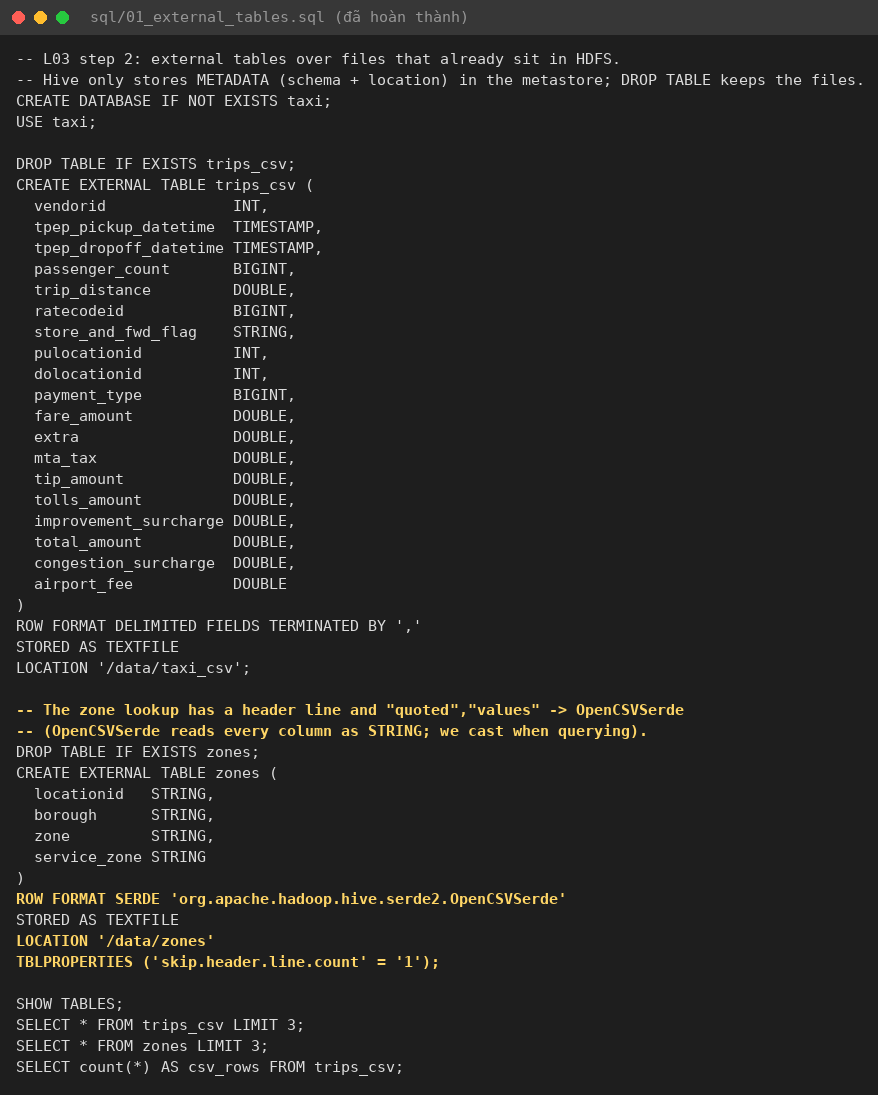
\includegraphics[keepaspectratio]{img/code_01_external_tables.png}}
\pandocbounded{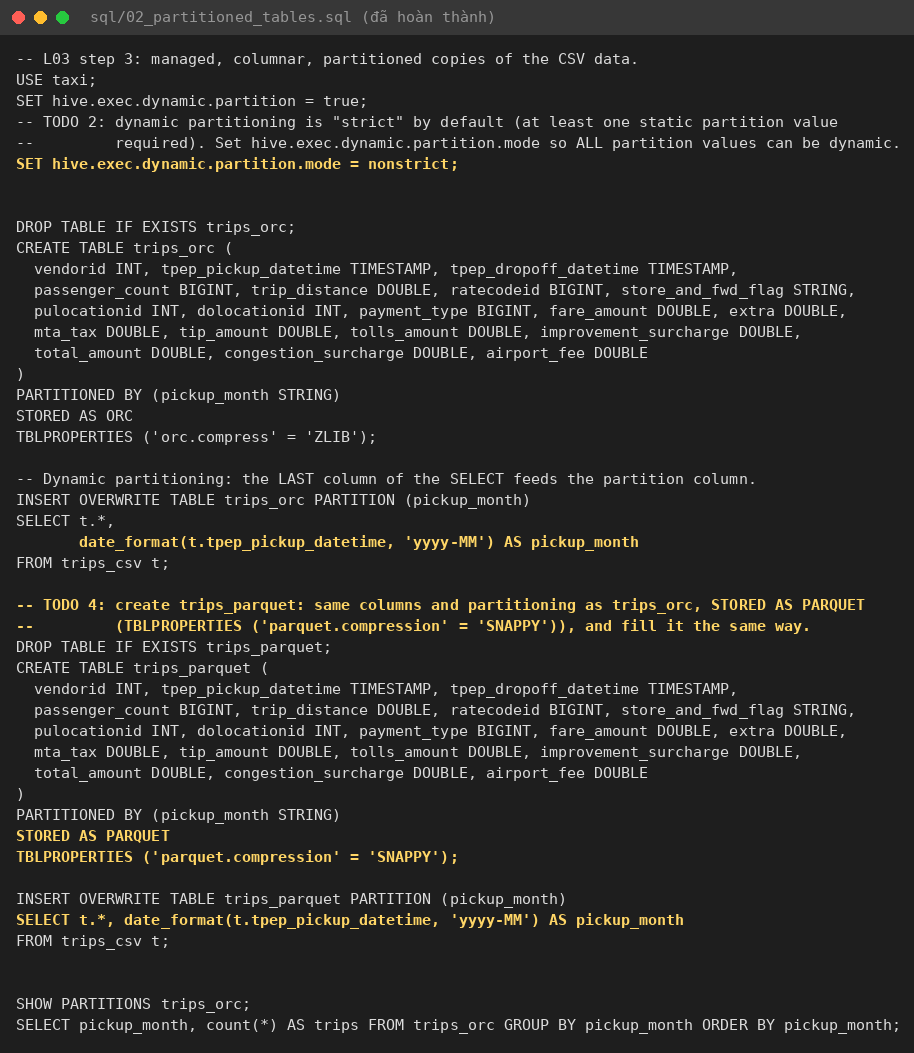
\includegraphics[keepaspectratio]{img/code_02_partitioned_tables.png}}
\pandocbounded{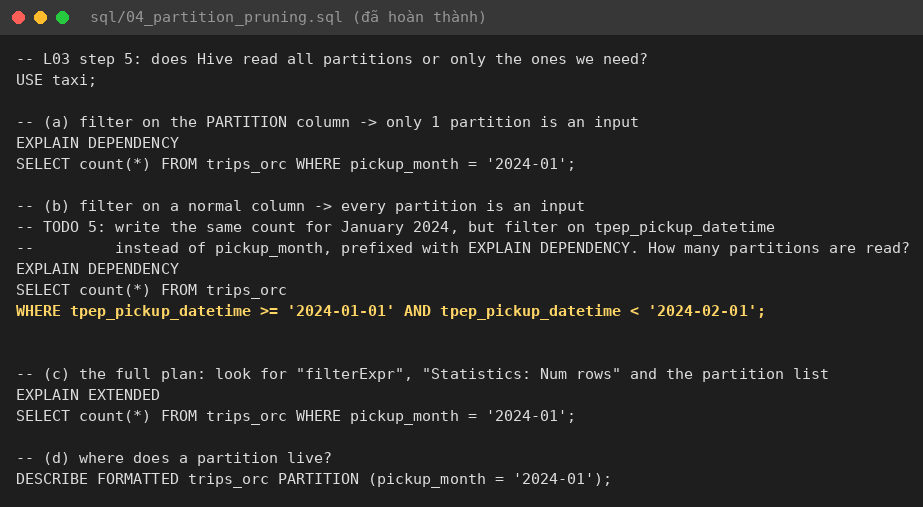
\includegraphics[keepaspectratio]{img/code_04_partition_pruning.png}}
\pandocbounded{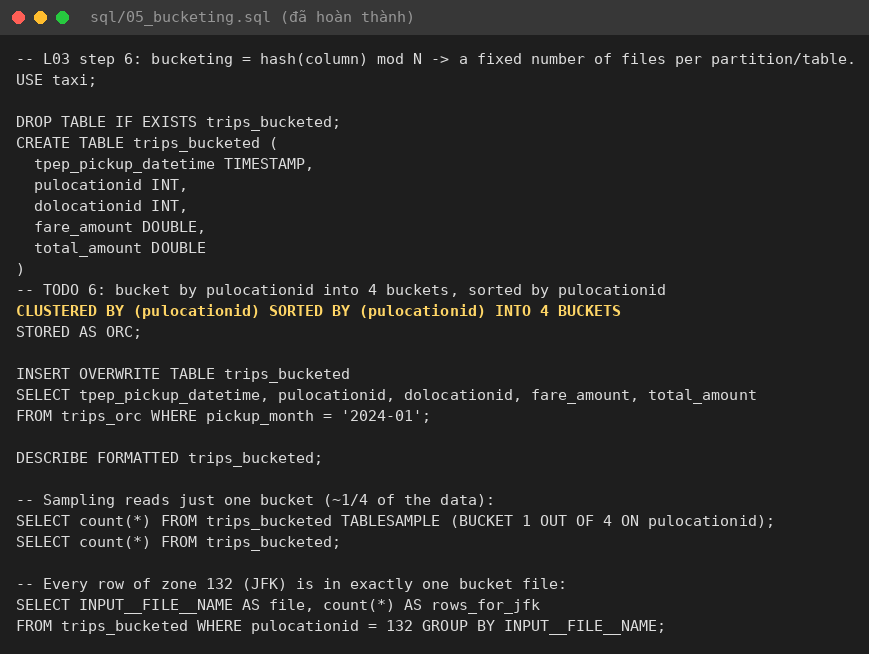
\includegraphics[keepaspectratio]{img/code_05_bucketing.png}}

\subsection{1--2. Khởi động stack và đưa CSV lên
HDFS}\label{khux1edfi-ux111ux1ed9ng-stack-vuxe0-ux111ux1b0a-csv-luxean-hdfs}

\pandocbounded{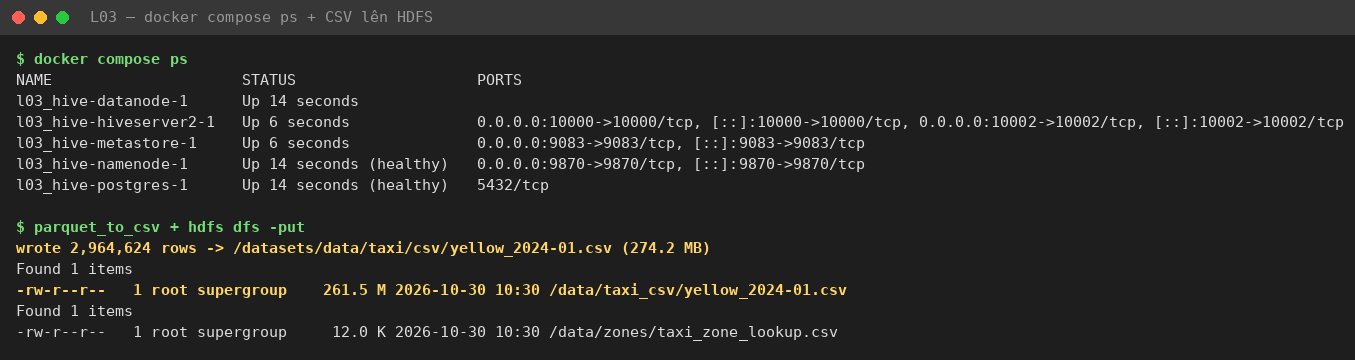
\includegraphics[keepaspectratio]{img/01_stack_and_upload.png}}
\pandocbounded{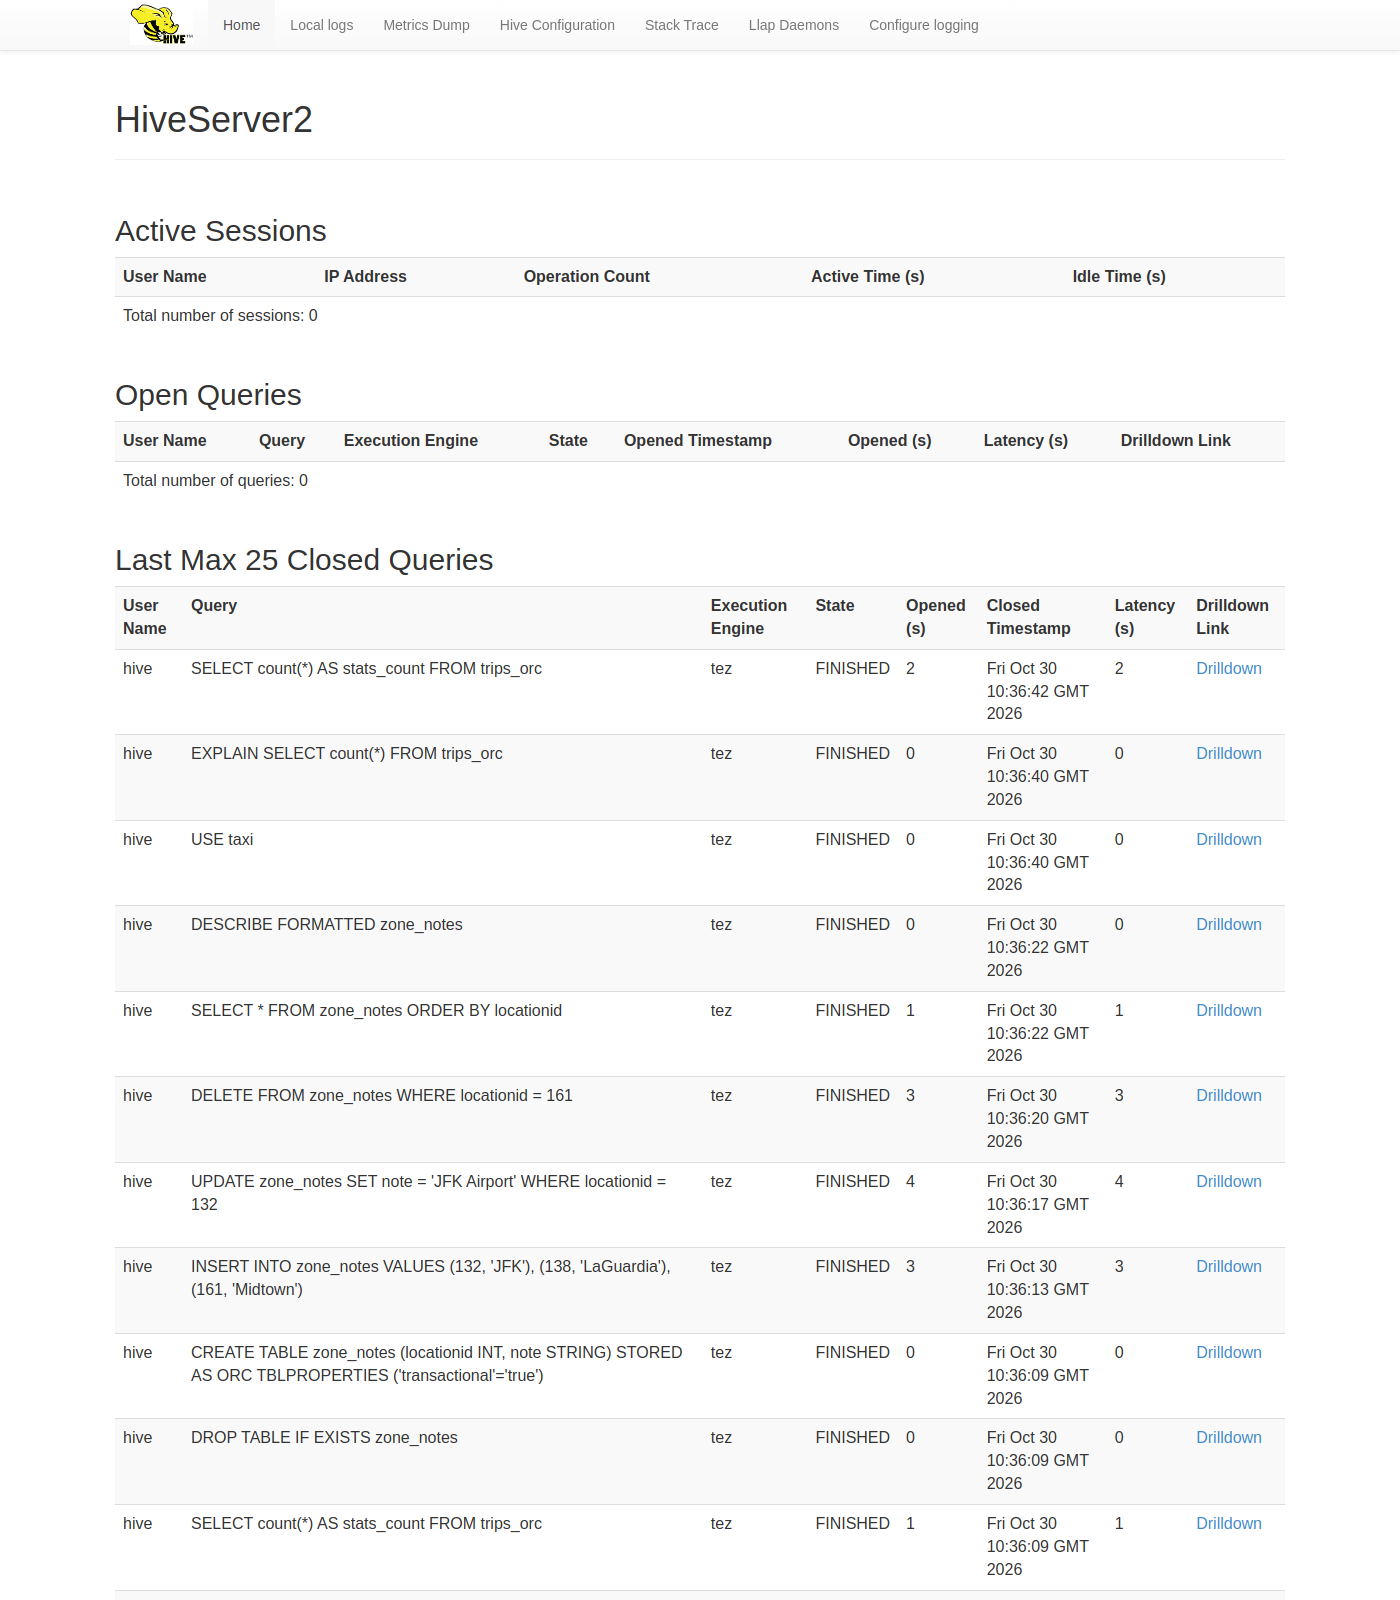
\includegraphics[keepaspectratio]{img/20_ui_hiveserver2_home.png}}

\subsection{3. External tables}\label{external-tables}

3 dòng mẫu, 3 zone
(\texttt{1\ \textbar{}\ EWR\ \textbar{}\ Newark\ Airport\ \textbar{}\ EWR}\ldots),
\texttt{csv\_rows\ =\ 2,964,624}. Metastore (Postgres) chỉ lưu tên bảng,
kiểu bảng, \texttt{LOCATION} và \texttt{INPUT\_FORMAT}:

\begin{figure}
\centering
\pandocbounded{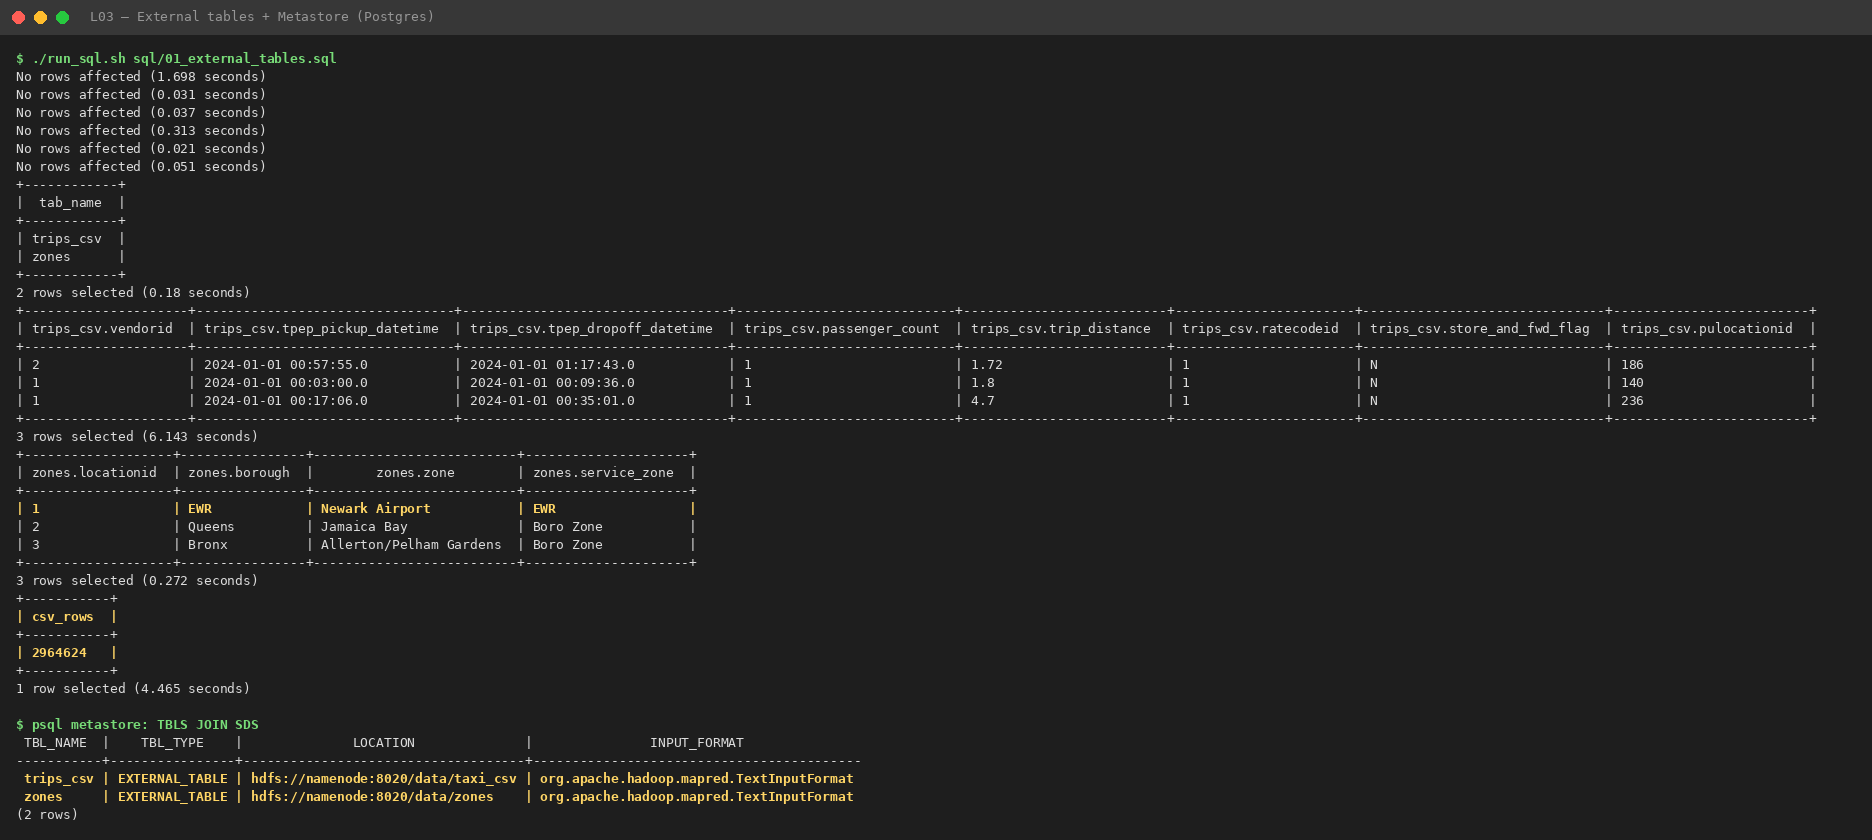
\includegraphics[keepaspectratio]{img/02_external_tables_and_metastore.png}}
\caption{external + metastore}
\end{figure}

\subsection{4. Bảng partition ORC và
Parquet}\label{bux1ea3ng-partition-orc-vuxe0-parquet}

INSERT OVERWRITE: ORC 42.8 s, Parquet 45.1 s (2,964,624 dòng mỗi bảng).
\texttt{SHOW\ PARTITIONS} cho \textbf{5 partition} (dữ liệu cả tháng có
thêm 2024-02 so với mẫu 1 triệu dòng):

\begin{longtable}[]{@{}ll@{}}
\toprule\noalign{}
pickup\_month & trips \\
\midrule\noalign{}
\endhead
\bottomrule\noalign{}
\endlastfoot
2002-12 & 2 \\
2009-01 & 3 \\
2023-12 & 10 \\
2024-01 & 2,964,606 \\
2024-02 & 3 \\
\end{longtable}

\pandocbounded{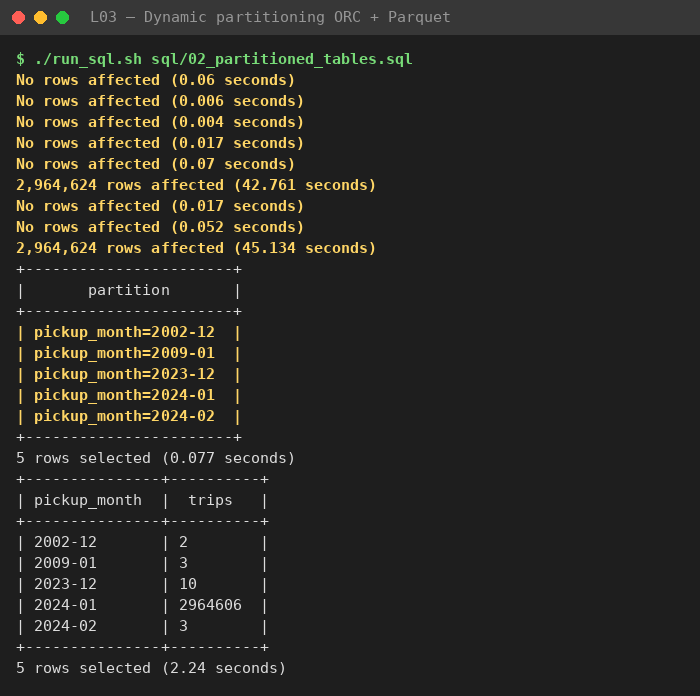
\includegraphics[keepaspectratio]{img/03_partitioned_tables.png}}
\pandocbounded{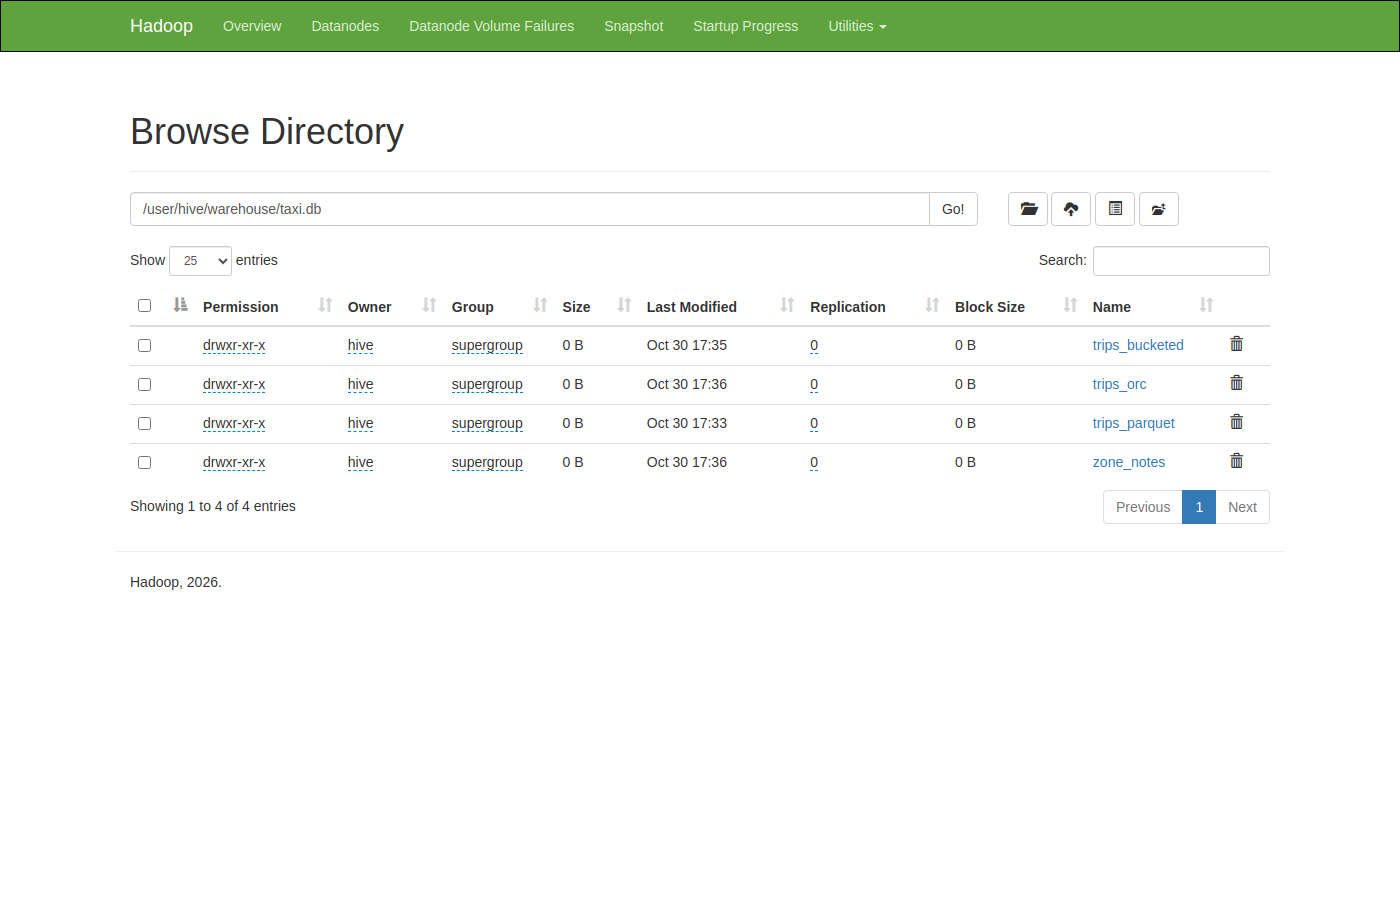
\includegraphics[keepaspectratio]{img/21_ui_hdfs_warehouse_taxi_db.png}}
\pandocbounded{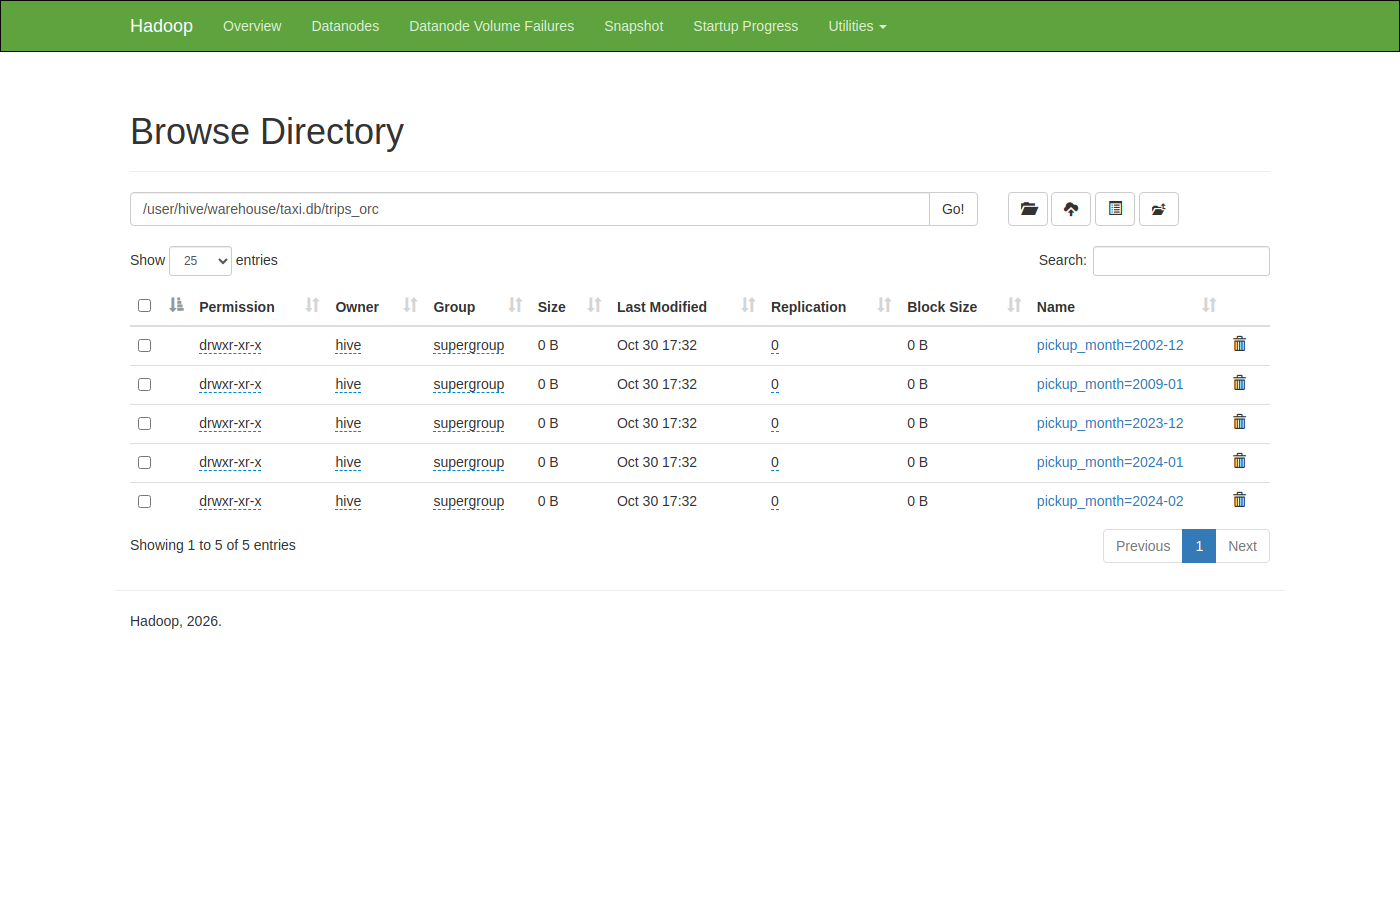
\includegraphics[keepaspectratio]{img/22_ui_hdfs_trips_orc_partitions.png}}

\texttt{DESCRIBE\ FORMATTED\ trips\_orc} cho thấy
\texttt{Table\ Type:\ EXTERNAL\_TABLE},
\texttt{TRANSLATED\_TO\_EXTERNAL=TRUE},
\texttt{external.table.purge=TRUE} (đúng hành vi Hive 4 với bảng
``managed'' không phải ACID).

\begin{figure}
\centering
\pandocbounded{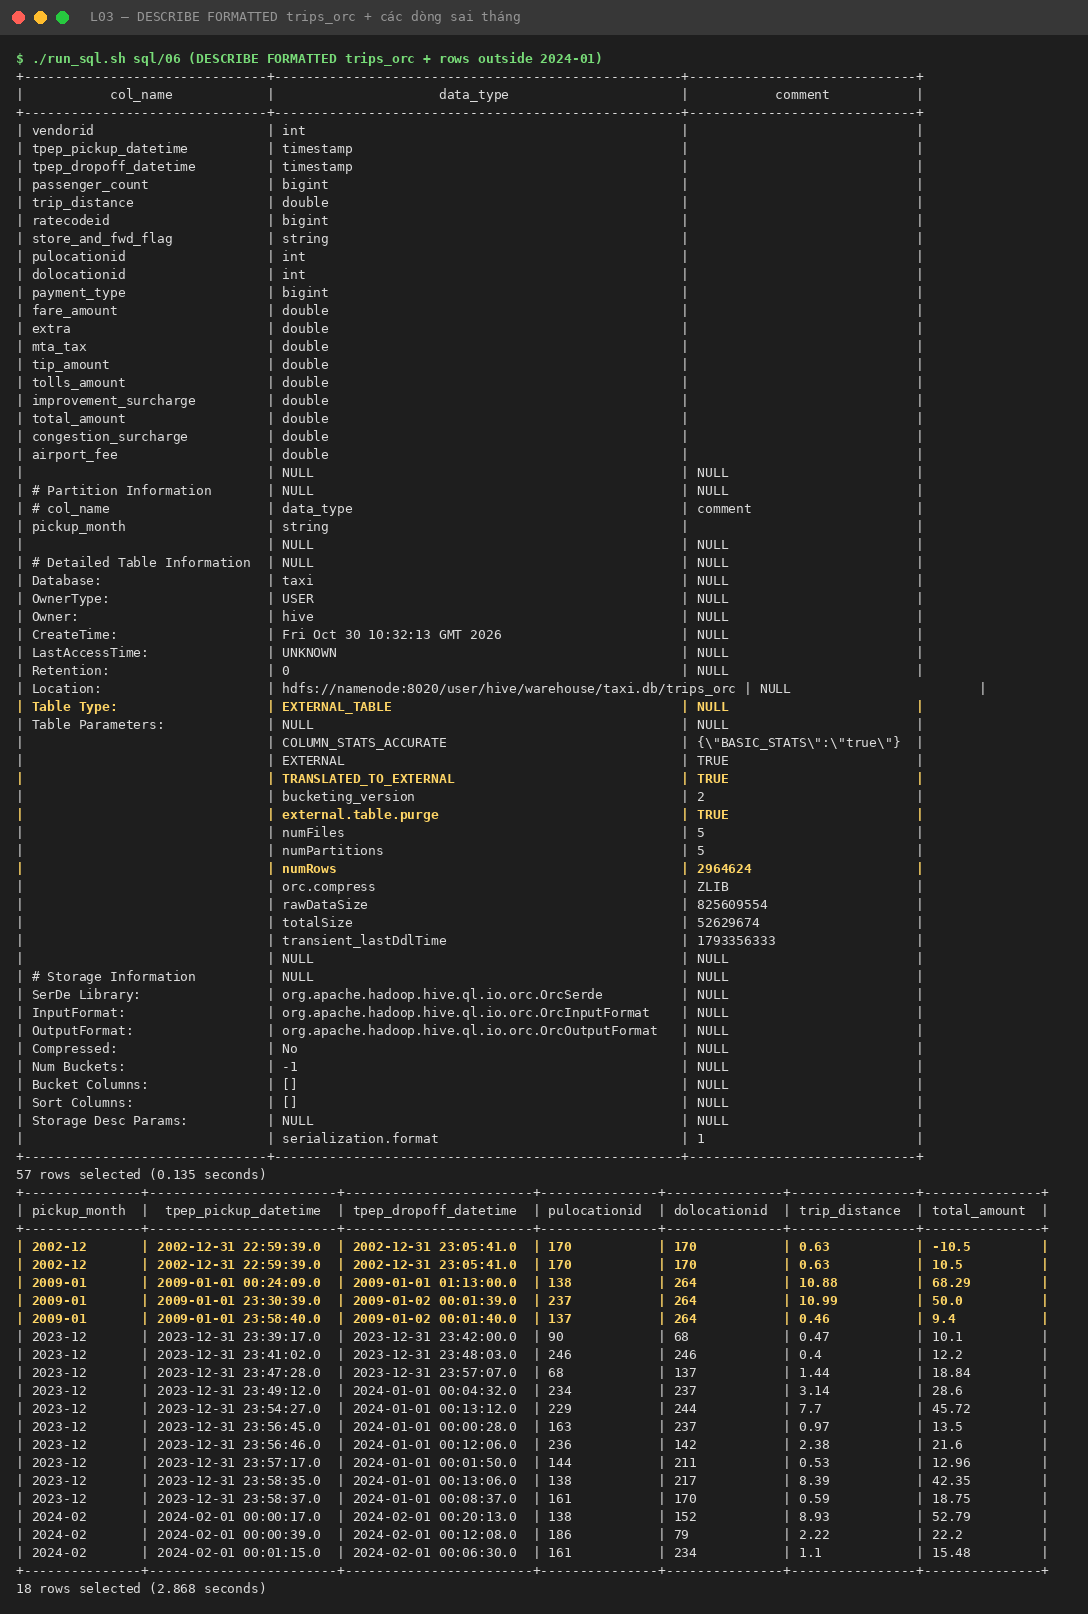
\includegraphics[keepaspectratio]{img/05_describe_formatted_and_bad_rows.png}}
\caption{describe + bad rows}
\end{figure}

\subsubsection{Bảng kích thước}\label{bux1ea3ng-kuxedch-thux1b0ux1edbc}

\begin{longtable}[]{@{}lll@{}}
\toprule\noalign{}
Định dạng & Kích thước (cả tháng, 2.96 triệu dòng) & So với CSV \\
\midrule\noalign{}
\endhead
\bottomrule\noalign{}
\endlastfoot
CSV (text) & 274,217,811 B (261.5 MiB) & 1× \\
ORC + ZLIB & 52,629,674 B (50.2 MiB) & \textbf{5.2× nhỏ hơn} \\
Parquet + Snappy & 65,305,645 B (62.3 MiB) & \textbf{4.2× nhỏ hơn} \\
ORC bucketed (chỉ 5 cột) & 25,271,072 B (24.1 MiB) & 10.9× \\
\end{longtable}

\begin{figure}
\centering
\pandocbounded{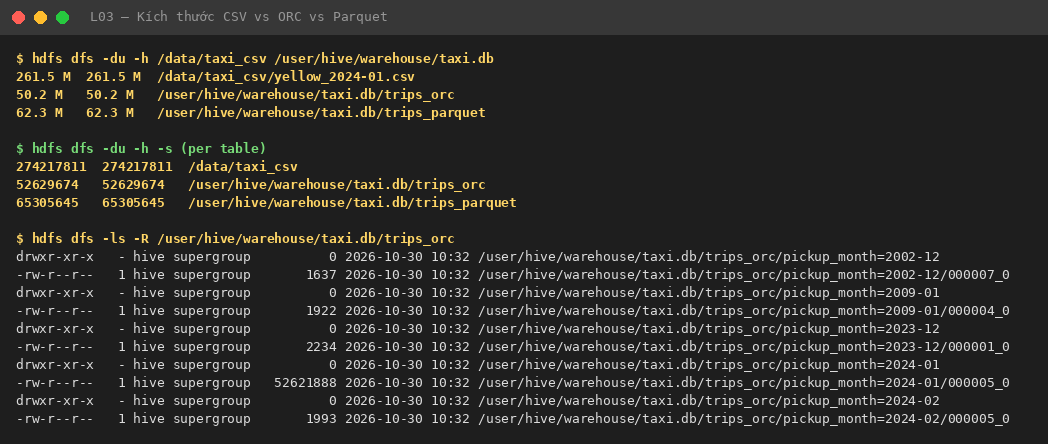
\includegraphics[keepaspectratio]{img/04_sizes_csv_orc_parquet.png}}
\caption{sizes}
\end{figure}

\subsection{5. CSV, ORC và Parquet: bảng thời gian (lần chạy thứ
2)}\label{csv-orc-vuxe0-parquet-bux1ea3ng-thux1eddi-gian-lux1ea7n-chux1ea1y-thux1ee9-2}

\begin{longtable}[]{@{}
  >{\raggedright\arraybackslash}p{(\linewidth - 6\tabcolsep) * \real{0.2500}}
  >{\raggedright\arraybackslash}p{(\linewidth - 6\tabcolsep) * \real{0.2500}}
  >{\raggedright\arraybackslash}p{(\linewidth - 6\tabcolsep) * \real{0.2500}}
  >{\raggedright\arraybackslash}p{(\linewidth - 6\tabcolsep) * \real{0.2500}}@{}}
\toprule\noalign{}
\begin{minipage}[b]{\linewidth}\raggedright
Query
\end{minipage} & \begin{minipage}[b]{\linewidth}\raggedright
CSV
\end{minipage} & \begin{minipage}[b]{\linewidth}\raggedright
ORC
\end{minipage} & \begin{minipage}[b]{\linewidth}\raggedright
Parquet
\end{minipage} \\
\midrule\noalign{}
\endhead
\bottomrule\noalign{}
\endlastfoot
Q1 top pickup zones tháng 01/2024 & \textbf{8.53 s} & \textbf{1.89 s} &
\textbf{1.62 s} \\
Q2 join \texttt{zones} theo borough (ORC) & & 2.66 s & \\
\end{longtable}

(Lần chạy 1: 9.22 / 1.99 / 1.77 s.) Q1 dòng đầu: zone \texttt{132} (JFK)
có \textbf{145,240 chuyến}, avg fare \textbf{59.40}; ba nguồn cho kết
quả giống hệt nhau. Q2: Manhattan 2,646,933 chuyến (\textbf{89.3 \%}),
Queens 273,125, Brooklyn 25,258\ldots{}

\begin{figure}
\centering
\pandocbounded{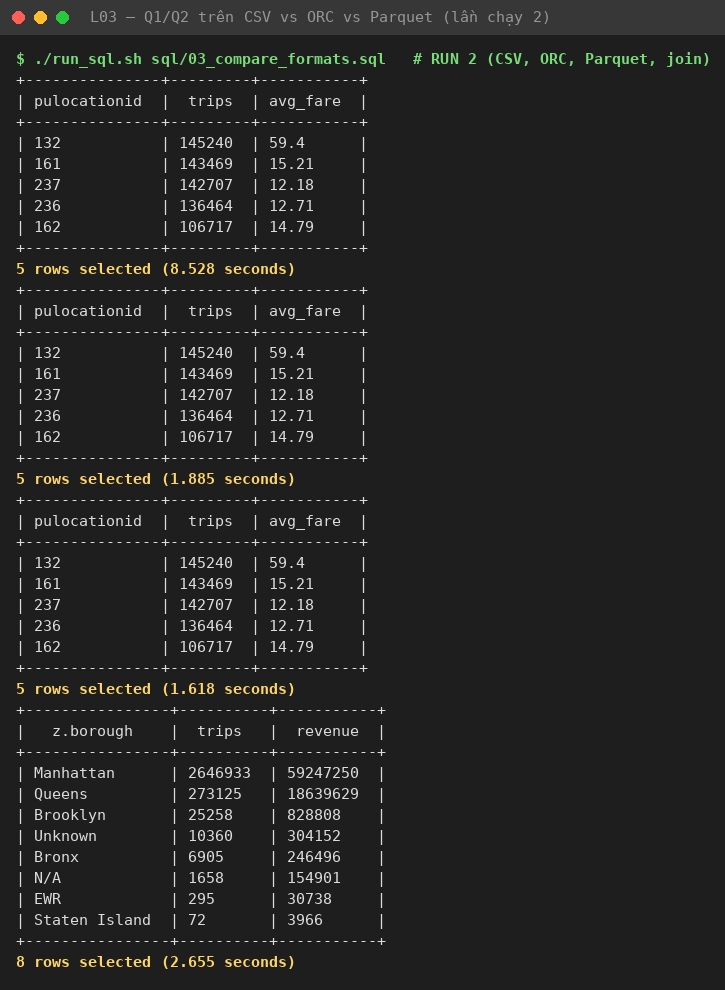
\includegraphics[keepaspectratio]{img/06_compare_formats_run2.png}}
\caption{compare}
\end{figure}

\subsection{6. Partition pruning}\label{partition-pruning}

\begin{itemize}
\tightlist
\item
  \begin{enumerate}
  \def\labelenumi{(\alph{enumi})}
  \tightlist
  \item
    \texttt{WHERE\ pickup\_month\ =\ \textquotesingle{}2024-01\textquotesingle{}}
    → \texttt{input\_partitions} chỉ có \textbf{1} partition.
  \end{enumerate}
\item
  \begin{enumerate}
  \def\labelenumi{(\alph{enumi})}
  \setcounter{enumi}{1}
  \tightlist
  \item
    TODO 5, \texttt{WHERE\ tpep\_pickup\_datetime} trong tháng 1 →
    \textbf{cả 5} partition là input (Hive không suy được partition từ
    cột thường).
  \end{enumerate}
\item
  \begin{enumerate}
  \def\labelenumi{(\alph{enumi})}
  \setcounter{enumi}{2}
  \tightlist
  \item
    \texttt{EXPLAIN\ EXTENDED}:
    \texttt{filterExpr:\ (pickup\_month\ =\ \textquotesingle{}2024-01\textquotesingle{})},
    \texttt{Path\ -\textgreater{}\ Alias} chỉ có
    \texttt{.../trips\_orc/pickup\_month=2024-01}.
  \end{enumerate}
\end{itemize}

\begin{figure}
\centering
\pandocbounded{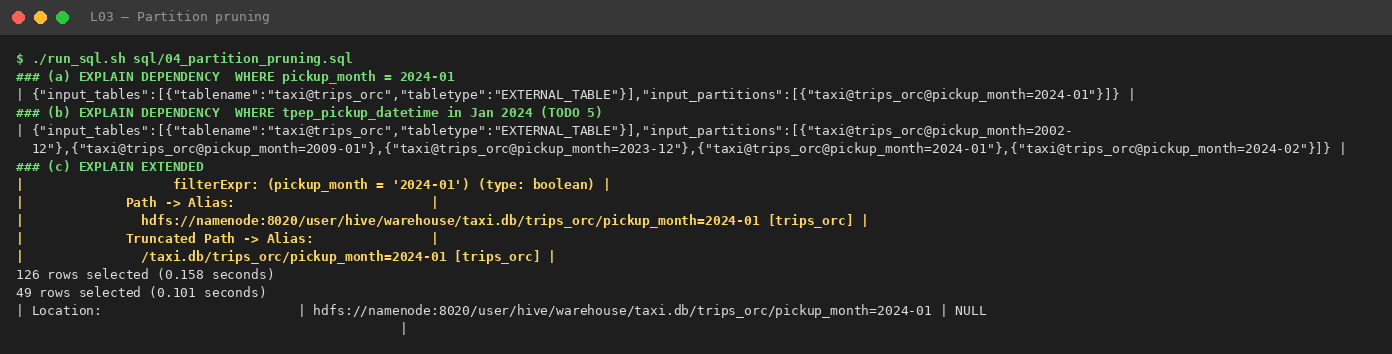
\includegraphics[keepaspectratio]{img/07_partition_pruning.png}}
\caption{pruning}
\end{figure}

\subsection{7. Bucketing}\label{bucketing}

Đúng \textbf{4 file} \texttt{000000\_0\ …\ 000003\_0}.
\texttt{TABLESAMPLE(BUCKET\ 1\ OUT\ OF\ 4)} = 619,893 dòng
(\textasciitilde21 \%, vì bucket theo hash nên không đều). Cả
\textbf{145,240 dòng JFK} đều nằm trong \textbf{một} file
\texttt{000002\_0} (vì vậy file này lớn nhất, 8.1 MB).

\pandocbounded{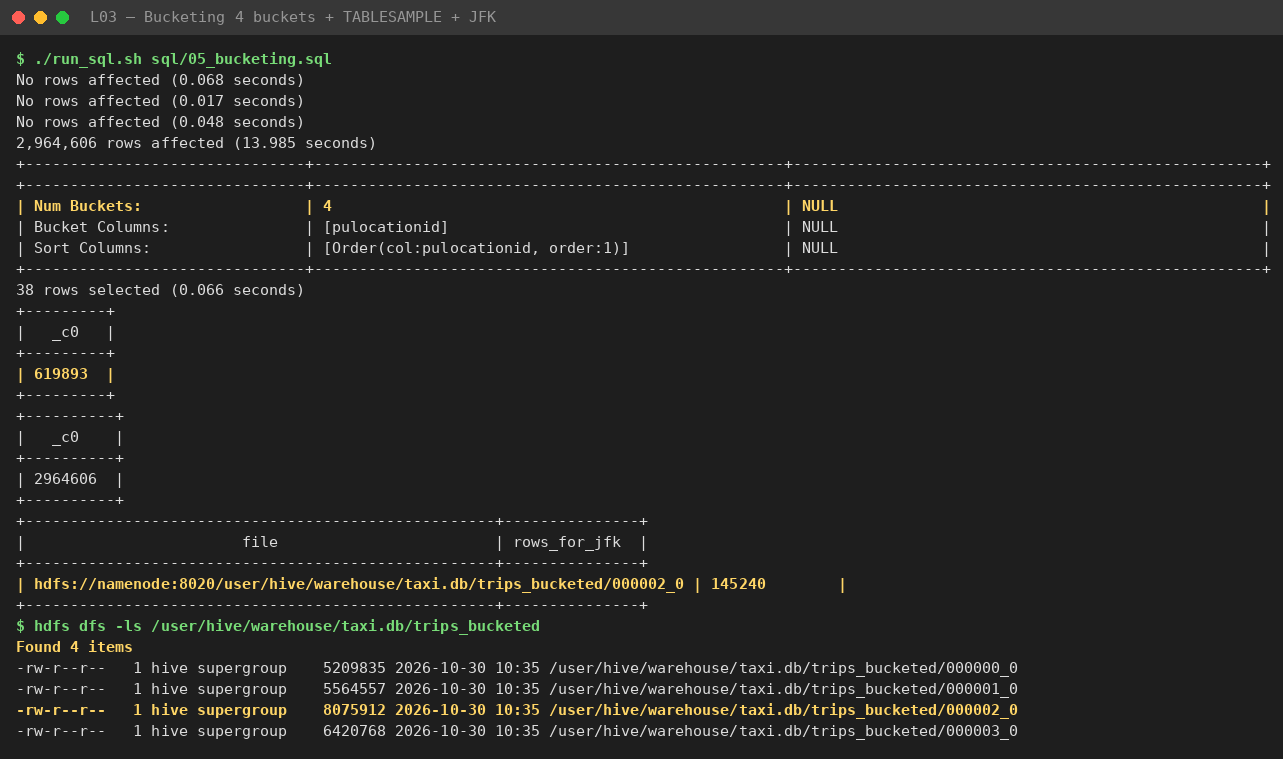
\includegraphics[keepaspectratio]{img/08_bucketing.png}}
\pandocbounded{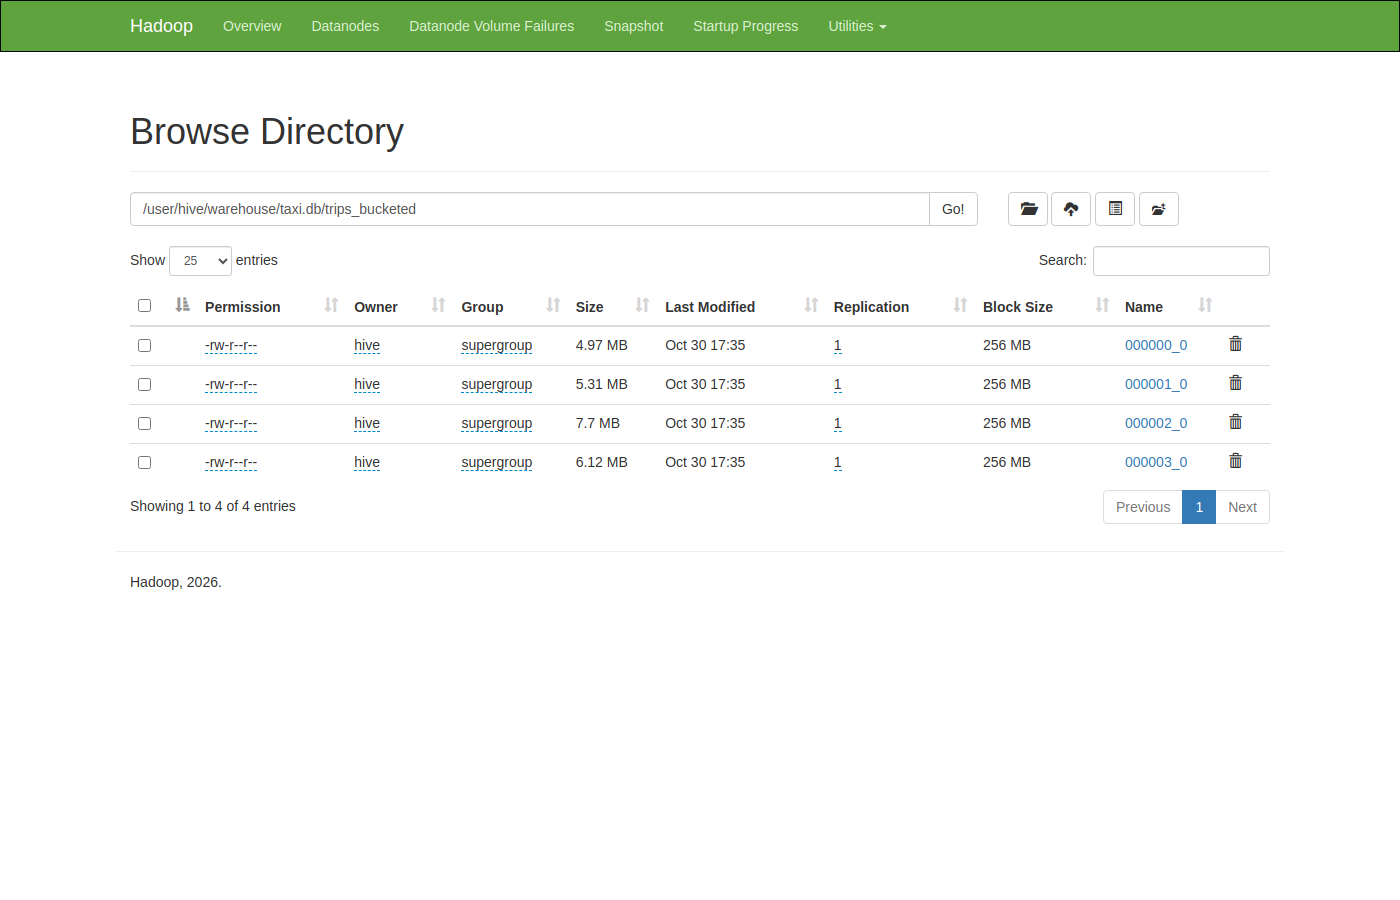
\includegraphics[keepaspectratio]{img/23_ui_hdfs_trips_bucketed_4files.png}}

\subsection{Stretch}\label{stretch}

\textbf{ACID.} \texttt{zone\_notes} với \texttt{transactional=true} là
\texttt{MANAGED\_TABLE} thật. Sau INSERT, UPDATE rồi DELETE, HDFS có
\texttt{delta\_0000001} (insert), \texttt{delete\_delta\_0000002} +
\texttt{delta\_0000002} (UPDATE = xoá + ghi lại) và
\texttt{delete\_delta\_0000003} (DELETE). Không file nào bị sửa tại chỗ;
reader merge các delta khi đọc, compaction gộp chúng về sau.

\textbf{Statistics.}
\texttt{ANALYZE\ ...\ COMPUTE\ STATISTICS\ FOR\ COLUMNS} mất 18.4 s. Sau
đó, với \texttt{hive.compute.query.using.stats=true}, \texttt{count(*)}
\textbf{vẫn chạy DAG Tez} (EXPLAIN vẫn có \texttt{TableScan},
\textasciitilde1.6--2.6 s). Lý do: \texttt{trips\_orc} thực chất là bảng
\textbf{EXTERNAL} (translated), và Hive không tin stats của bảng
external để trả lời thay cho việc quét, vì file có thể bị thay đổi ngoài
Hive. Với bảng managed/ACID, câu trả lời sẽ lấy thẳng từ metastore (chỉ
còn Fetch, không có job).

\pandocbounded{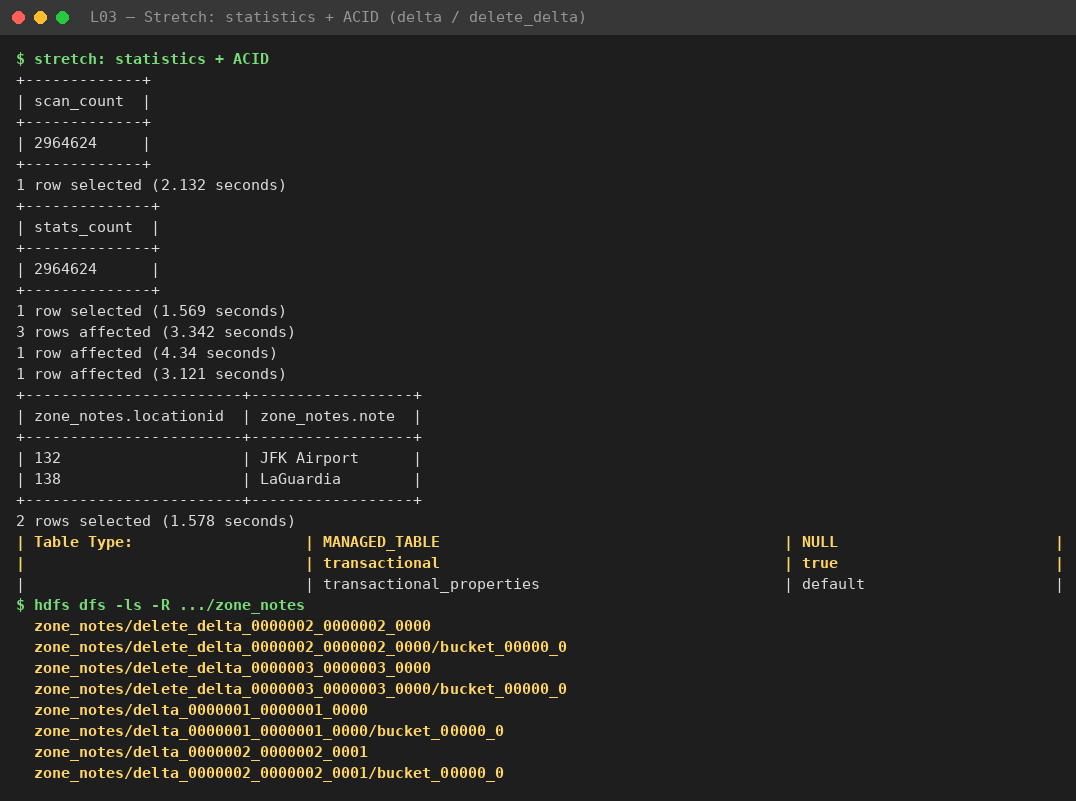
\includegraphics[keepaspectratio]{img/09_stretch_stats_acid.png}}
\pandocbounded{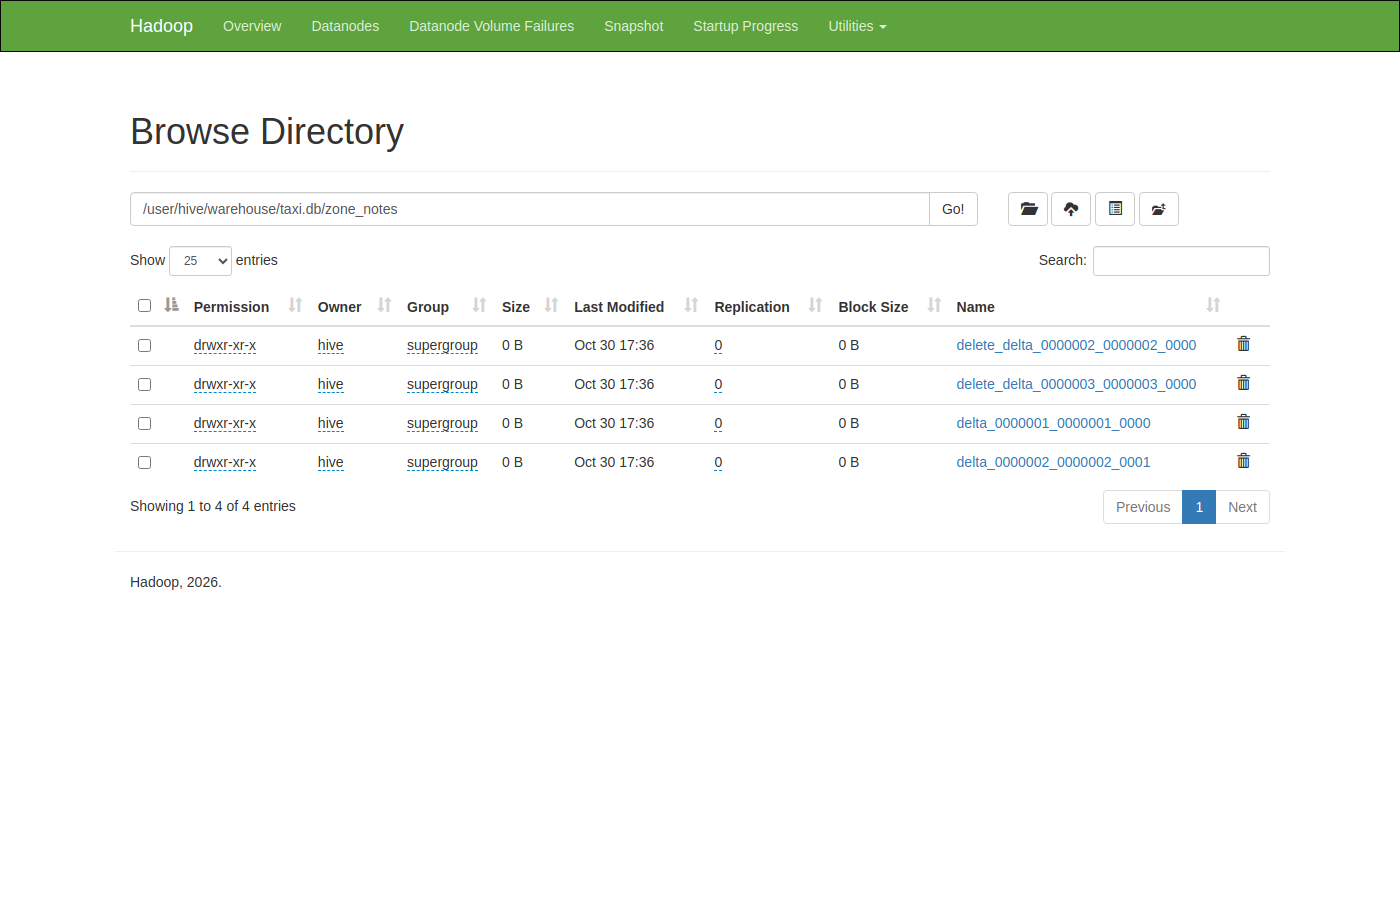
\includegraphics[keepaspectratio]{img/24_ui_hdfs_zone_notes_acid_deltas.png}}

\subsection{Trả lời checkpoint}\label{trux1ea3-lux1eddi-checkpoint}

\textbf{Q1. Metastore lưu gì, HDFS lưu gì? DROP TABLE thì sao?}
\textbf{Metastore} (bảng \texttt{TBLS}, \texttt{SDS},
\texttt{PARTITIONS}\ldots{} trong Postgres): database, tên bảng, cột và
kiểu, SerDe, input/output format, kiểu bảng, \textbf{LOCATION} của bảng
và của từng partition, giá trị partition, thống kê (numRows,
totalSize\ldots), trạng thái ACID/transaction. \textbf{HDFS} chỉ chứa
file dữ liệu. \texttt{DROP\ TABLE\ trips\_csv} (external): chỉ xoá
metadata, file trong \texttt{/data/taxi\_csv} vẫn còn.
\texttt{DROP\ TABLE\ trips\_orc} (external +
\texttt{external.table.purge=TRUE}): xoá metadata \textbf{và} thư mục
\texttt{/user/hive/warehouse/taxi.db/trips\_orc}.

\textbf{Q3. Vì sao ORC/Parquet nhỏ hơn CSV 4--5 lần?} (thực đo 5.2× và
4.2×) (a) \textbf{Lưu theo cột}: giá trị cùng kiểu, cùng cột nằm cạnh
nhau nên các encoding dictionary, RLE, delta, bit-packing rất hiệu quả
(\texttt{vendorid}, \texttt{payment\_type}, \texttt{ratecodeid} chỉ có
vài giá trị khác nhau). (b) \textbf{Kiểu nhị phân + nén} (ZLIB/Snappy)
thay cho chữ số dạng text và dấu phân cách: một timestamp là 8 byte số
thay vì chuỗi 19 ký tự. ORC + ZLIB nén mạnh hơn Parquet + Snappy (Snappy
ưu tiên tốc độ hơn tỉ lệ nén).

\textbf{Q4. Vì sao Q1 nhanh hơn trên ORC/Parquet?} (8.53 s → 1.89 / 1.62
s, nhanh \textasciitilde4.5--5×) * \textbf{Column pruning}: Q1 chỉ cần
2--3 trong 19 cột (\texttt{pulocationid}, \texttt{fare\_amount}, cột
partition). ORC/Parquet chỉ đọc các column chunk đó, còn CSV phải đọc và
parse \textbf{toàn bộ} 274 MB, từng dòng. * \textbf{Partition pruning}:
với ORC/Parquet, filter nằm trên \texttt{pickup\_month}, nên Hive chỉ mở
thư mục \texttt{pickup\_month=2024-01} (đã chứng minh bằng EXPLAIN
DEPENDENCY, 1 so với 5 partition). Bảng CSV không có partition nên phải
quét hết rồi lọc theo timestamp. * \textbf{Predicate pushdown / min-max
statistics}: mỗi stripe/row group lưu min/max và có row index, nên
reader bỏ qua được các khối không thể khớp điều kiện. * Ngoài ra, reader
ORC/Parquet được \textbf{vectorized} (xử lý theo batch 1,024 dòng) và
không tốn công parse text thành số.

\textbf{Q6. Partition theo \texttt{pulocationid} + ngày? Theo
\texttt{tpep\_pickup\_datetime}?} \texttt{pulocationid} × ngày ≈ 265 ×
31 ≈ \textbf{8,000 partition mỗi tháng}, mỗi partition chỉ có một file
vài KB đến vài trăm KB. Đây là \textbf{small files problem}: NameNode
phải giữ hàng chục nghìn object trong heap, \textbf{Metastore} phải lưu
hàng nghìn dòng \texttt{PARTITIONS}/\texttt{SDS} (query planning chậm vì
phải liệt kê và lấy metadata partition), và mỗi file nhỏ thành một
split/task riêng nên overhead lấn át thời gian xử lý thật. Partition
theo timestamp gốc thì gần như \textbf{mỗi giây một partition}: hàng
triệu thư mục, file vài trăm byte, metastore và NameNode quá tải. Nguyên
tắc: partition theo cột có cardinality thấp mà query hay lọc, mỗi
partition nên chứa từ hàng trăm MB đến khoảng 1 GB.

\textbf{Q7. Partitioning hay bucketing? Vì sao bucketing có số file cố
định?} \textbf{Partitioning} tạo thư mục theo \textbf{giá trị} cột, dùng
cho cột cardinality thấp mà query hay lọc (ngày, tháng, quốc gia), để bỏ
qua cả thư mục khi đọc. \textbf{Bucketing} chia dữ liệu theo
\texttt{hash(col)\ mod\ N} vào N file, dùng cho cột cardinality cao (id,
\texttt{pulocationid}). Nó cho phép sampling (\texttt{TABLESAMPLE}),
bucket map join hoặc sort-merge-bucket join, và tránh shuffle khi hai
bảng được bucket giống nhau trên khoá join. Số file cố định vì \textbf{N
được chốt trong DDL} (\texttt{INTO\ 4\ BUCKETS}): mỗi dòng đi vào đúng
bucket \texttt{hash\ mod\ 4} bất kể dữ liệu nhiều hay ít (thực nghiệm:
đúng 4 file, mọi dòng JFK nằm trong \texttt{000002\_0}).

\textbf{Q2.} Trong file trips, \texttt{ROW\ FORMAT\ DELIMITED}
(LazySimpleSerDe) chỉ tách theo dấu phẩy, đủ dùng vì không có ngoặc kép
hay header. File zones có header và
\texttt{"giá\ trị\ trong\ ngoặc\ kép"} (ví dụ
\texttt{"Allerton/Pelham\ Gardens"}), nên cần \texttt{OpenCSVSerde}.
Nhược điểm của nó: \textbf{mọi cột đều là STRING} (phải tự CAST, như
\texttt{CAST(z.locationid\ AS\ INT)} trong Q2), parse chậm hơn, không xử
lý NULL đặc biệt.

\textbf{Q5.} Partition tĩnh ghi giá trị ngay trong câu lệnh
(\texttt{PARTITION\ (pickup\_month=\textquotesingle{}2024-01\textquotesingle{})}).
Partition động lấy giá trị từ dữ liệu (cột cuối của SELECT). Mặc định là
\texttt{strict} (bắt buộc ít nhất một giá trị tĩnh) để một câu query lỗi
không vô tình tạo hàng nghìn partition, file và object trong metastore.
Lab đã thấy điều này ở quy mô nhỏ: các dòng 2002/2009 sinh ra partition
``lạ''.

\textbf{Q8.} Có 18 dòng ngoài tháng 01/2024: 2 dòng 2002-12-31 (một cặp
+10.5/−10.5, tức một chuyến bị hoàn tiền), 3 dòng 2009-01-01, 10 dòng
2023-12-31 23:39--23:58 (chuyến bắt đầu trước nửa đêm giao thừa) và 3
dòng 2024-02-01 00:00 (chuyến bắt đầu ngay sau nửa đêm). Các dòng năm
2002/2009 là lỗi đồng hồ thiết bị, còn các dòng 2023-12 và 2024-02 là
chuyến thật nằm ở biên tháng. Trong pipeline thật: kiểm tra event time
so với tháng của file nguồn; đưa dòng ngoài khoảng hợp lệ vào bảng
\textbf{quarantine/rejected} kèm lý do và đếm/cảnh báo; các dòng biên
tháng hợp lệ thì ghi vào đúng partition (hoặc giữ lại theo tháng của
file); không để dynamic partitioning âm thầm tạo partition rác.

\end{document}
